% ============================================================
% SQLI-01
% ============================================================

\subsection*{SQL Injection -- Authentication Bypass (Login Endpoint) (SQLI-01)}

\begin{table}[H]
\centering
\begin{tabular}{|l|p{10cm}|}
\hline
\textbf{Finding ID} & SQLI-01 \\
\hline
\textbf{Severity} & Critical \\
\hline
\textbf{CVSS 3.1 Score} & 9.8 (Critical) \\
\hline
\textbf{CVSS Vector} & \texttt{AV:N/AC:L/PR:N/UI:N/S:U/C:H/I:H/A:H} \\
\hline
\textbf{Status} & Confirmed \\
\hline
\textbf{OWASP Category} & A03:2021 -- Injection \\
\hline
\textbf{CWE} & CWE-89 -- Improper Neutralization of Special
Elements used in an SQL Command (SQL Injection) \\
\hline
\textbf{Affected Endpoint} & \texttt{POST /rest/user/login} \\
\hline
\textbf{Affected Parameter} & \texttt{email} \\
\hline
\end{tabular}
\caption{SQL Injection -- Authentication Bypass finding details}
\end{table}

\subsubsection*{Description}

The login function was found to be vulnerable to SQL Injection
through the \texttt{email} parameter.

A SQL Injection payload was entered into the login form. The
application accepted the input and allowed authentication without
using valid administrator credentials.

This shows that user input is being used unsafely in the login
process. An attacker can use this weakness to bypass the login
controls.

\subsubsection*{Methodology}

The login functionality was tested manually using the application
and Burp Suite.

A SQL Injection payload was entered into the \texttt{email}
parameter while an arbitrary password was supplied. The resulting
HTTP request and server response were then inspected using Burp
Suite.

Successful authentication and access to the administrator session
were used as the primary evidence for confirming the vulnerability.

\subsubsection*{Steps to Reproduce}

\begin{enumerate}

    \item Navigate to
    \texttt{http://127.0.0.1:3000/\#/login}.

    \item Enter the following payload in the
    \textbf{email} field:

    \begin{lstlisting}
user' or 1=1--
    \end{lstlisting}

    \item Enter any value in the password field.

    \item Submit the login form.

    \item Capture the request using Burp Suite and verify that the
    request is sent to \texttt{POST /rest/user/login}.

    \item Observe the server response. The response returns
    \texttt{HTTP/1.1 200 OK} and an authentication token.

    \item Verify that the application logs in as the administrator
    account.

\end{enumerate}

\subsubsection*{Evidence}

\begin{figure}[H]
    \centering
    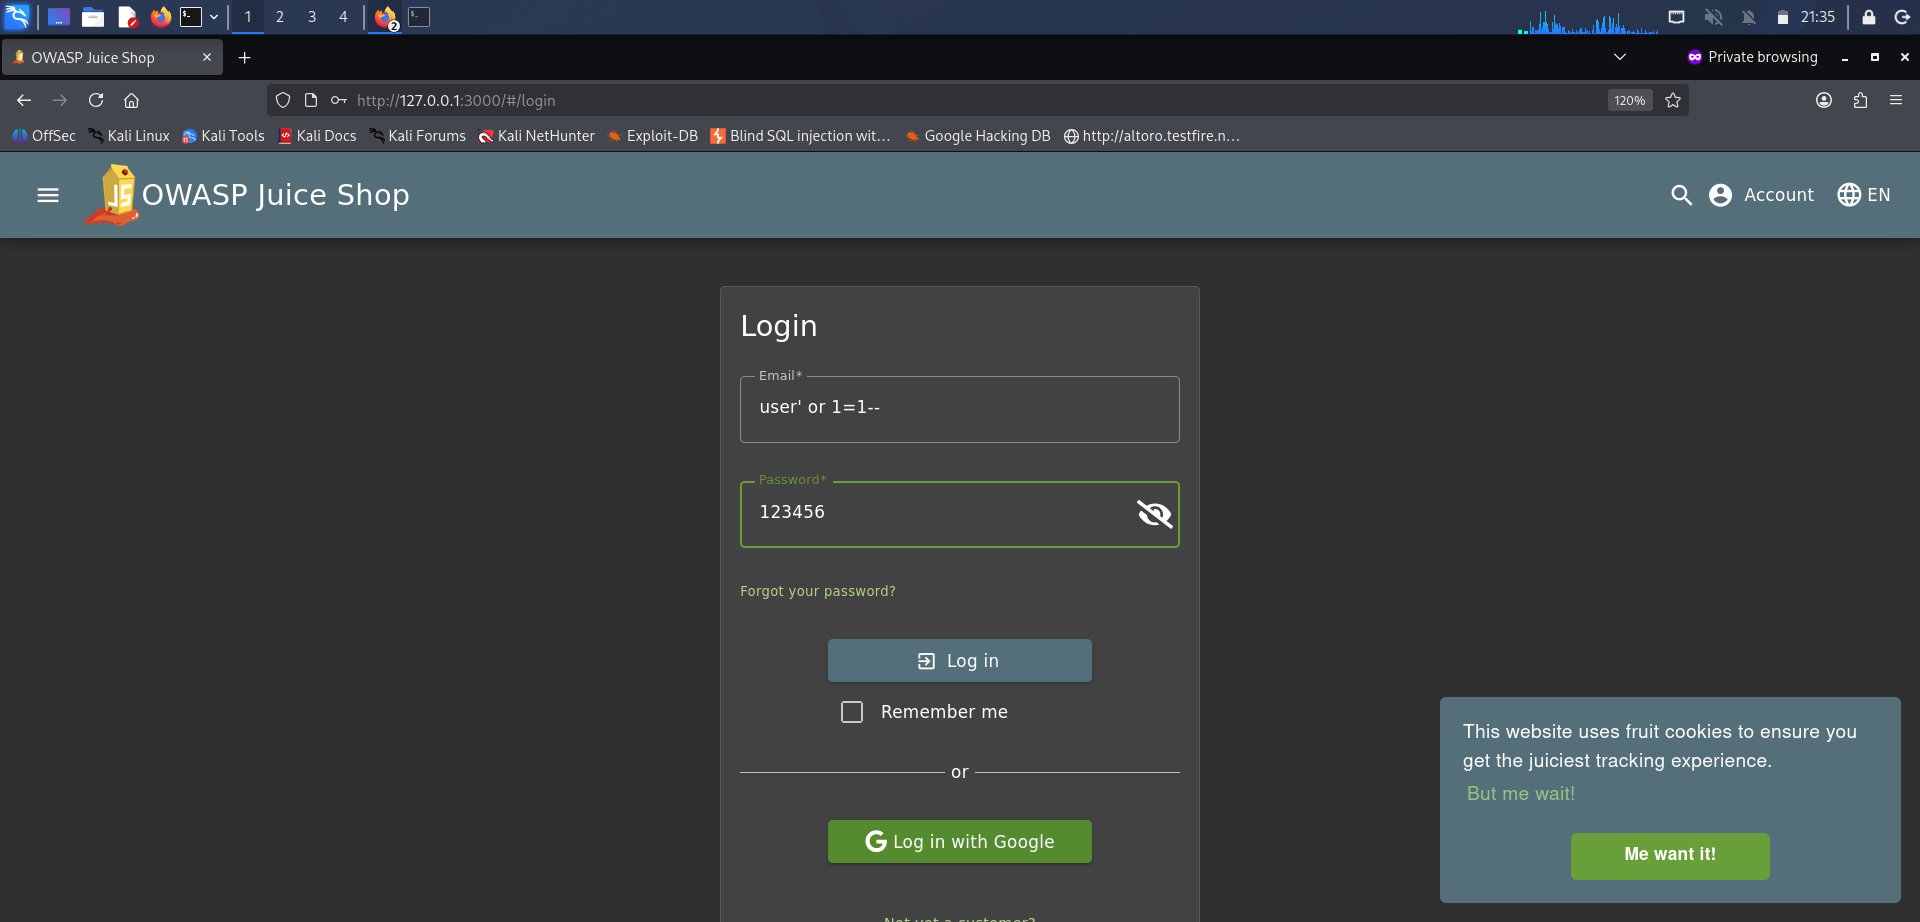
\includegraphics[width=0.8\textwidth]
    {evidence/phase4/sqli-1/sqli01-01-payload-injected-login-form.png}
    \caption{SQL Injection payload entered into the login form}
\end{figure}

\begin{figure}[H]
    \centering
    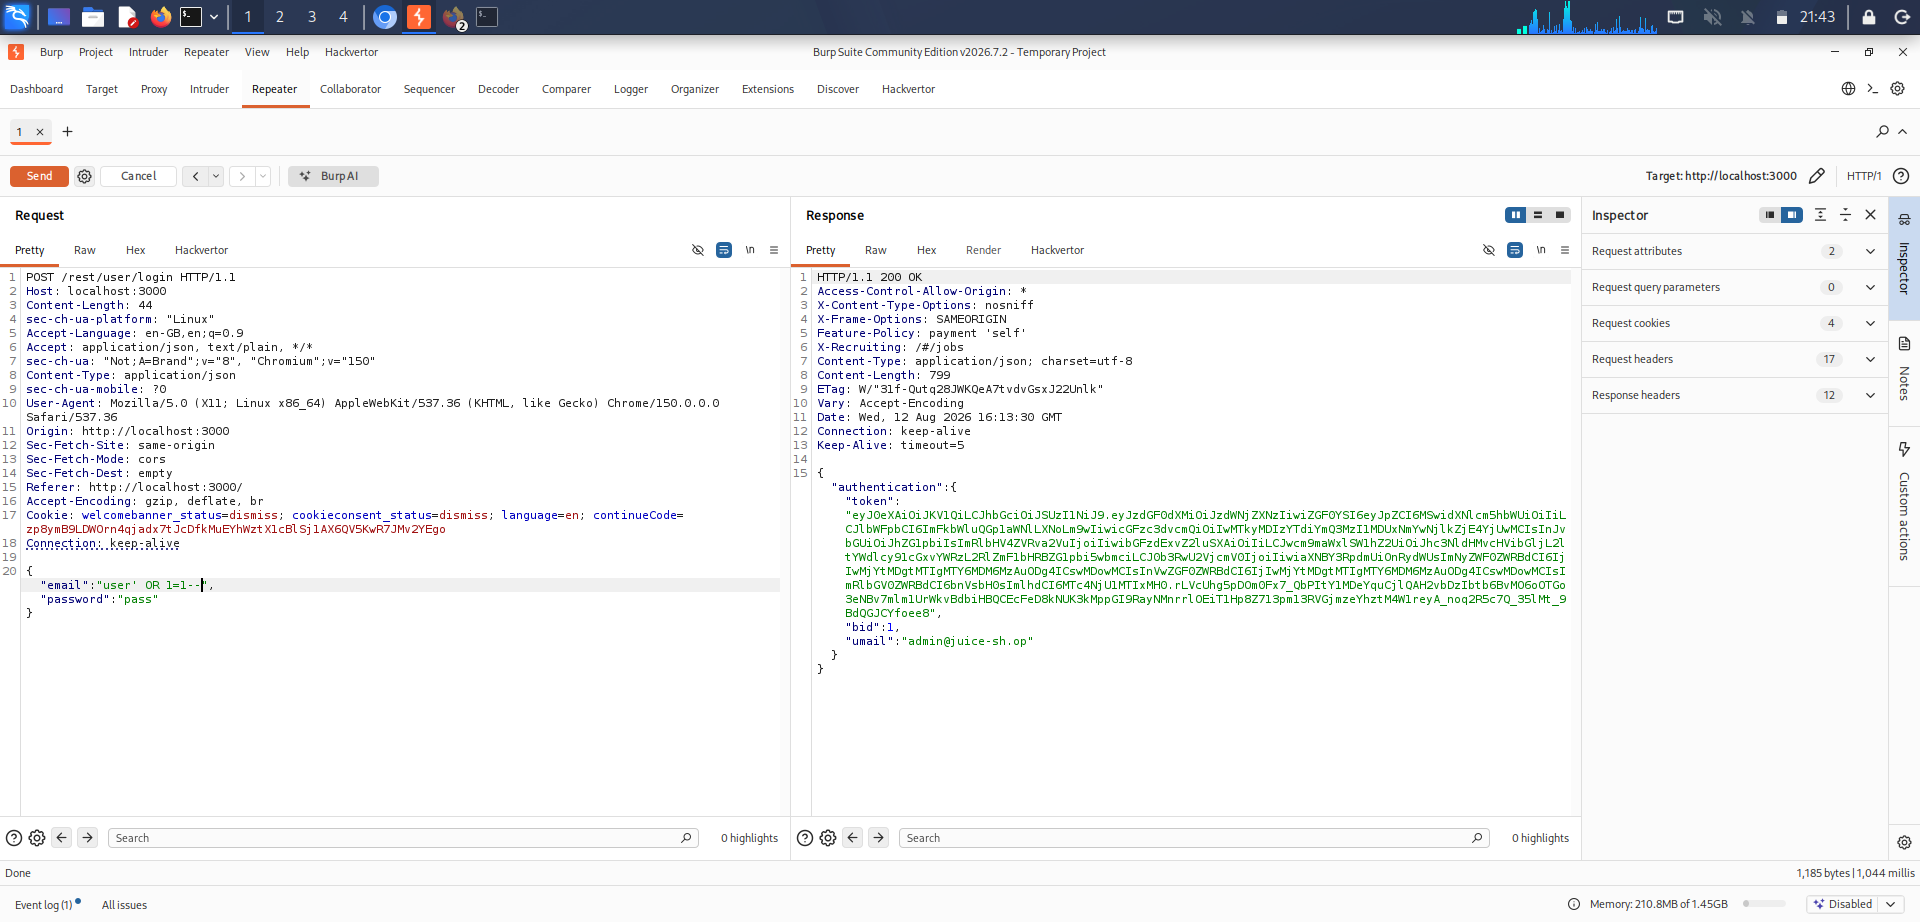
\includegraphics[width=0.8\textwidth]
    {evidence/phase4/sqli-1/sqli01-02-burp-request-response.png}
    \caption{Burp Suite request and response showing the injected input}
\end{figure}

\begin{figure}[H]
    \centering
    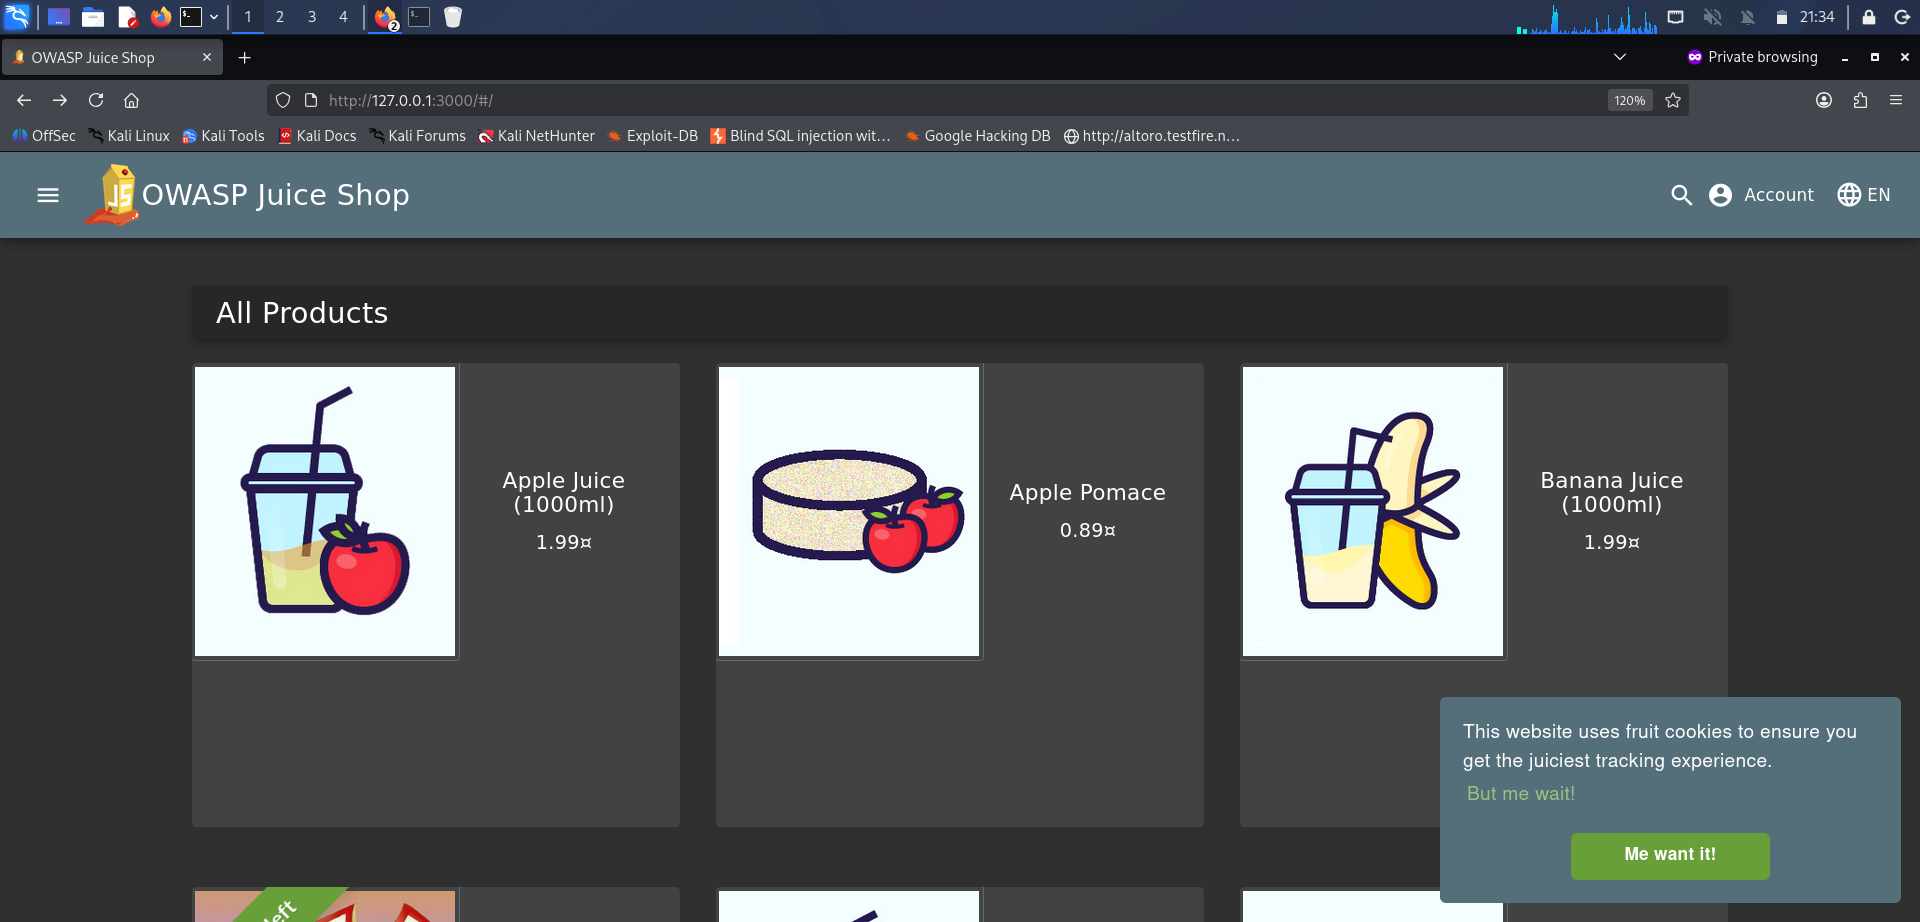
\includegraphics[width=0.8\textwidth]
    {evidence/phase4/sqli-1/sqli01-03-admin-login-success.png}
    \caption{Successful login as the administrator account}
\end{figure}

\begin{figure}[H]
    \centering
    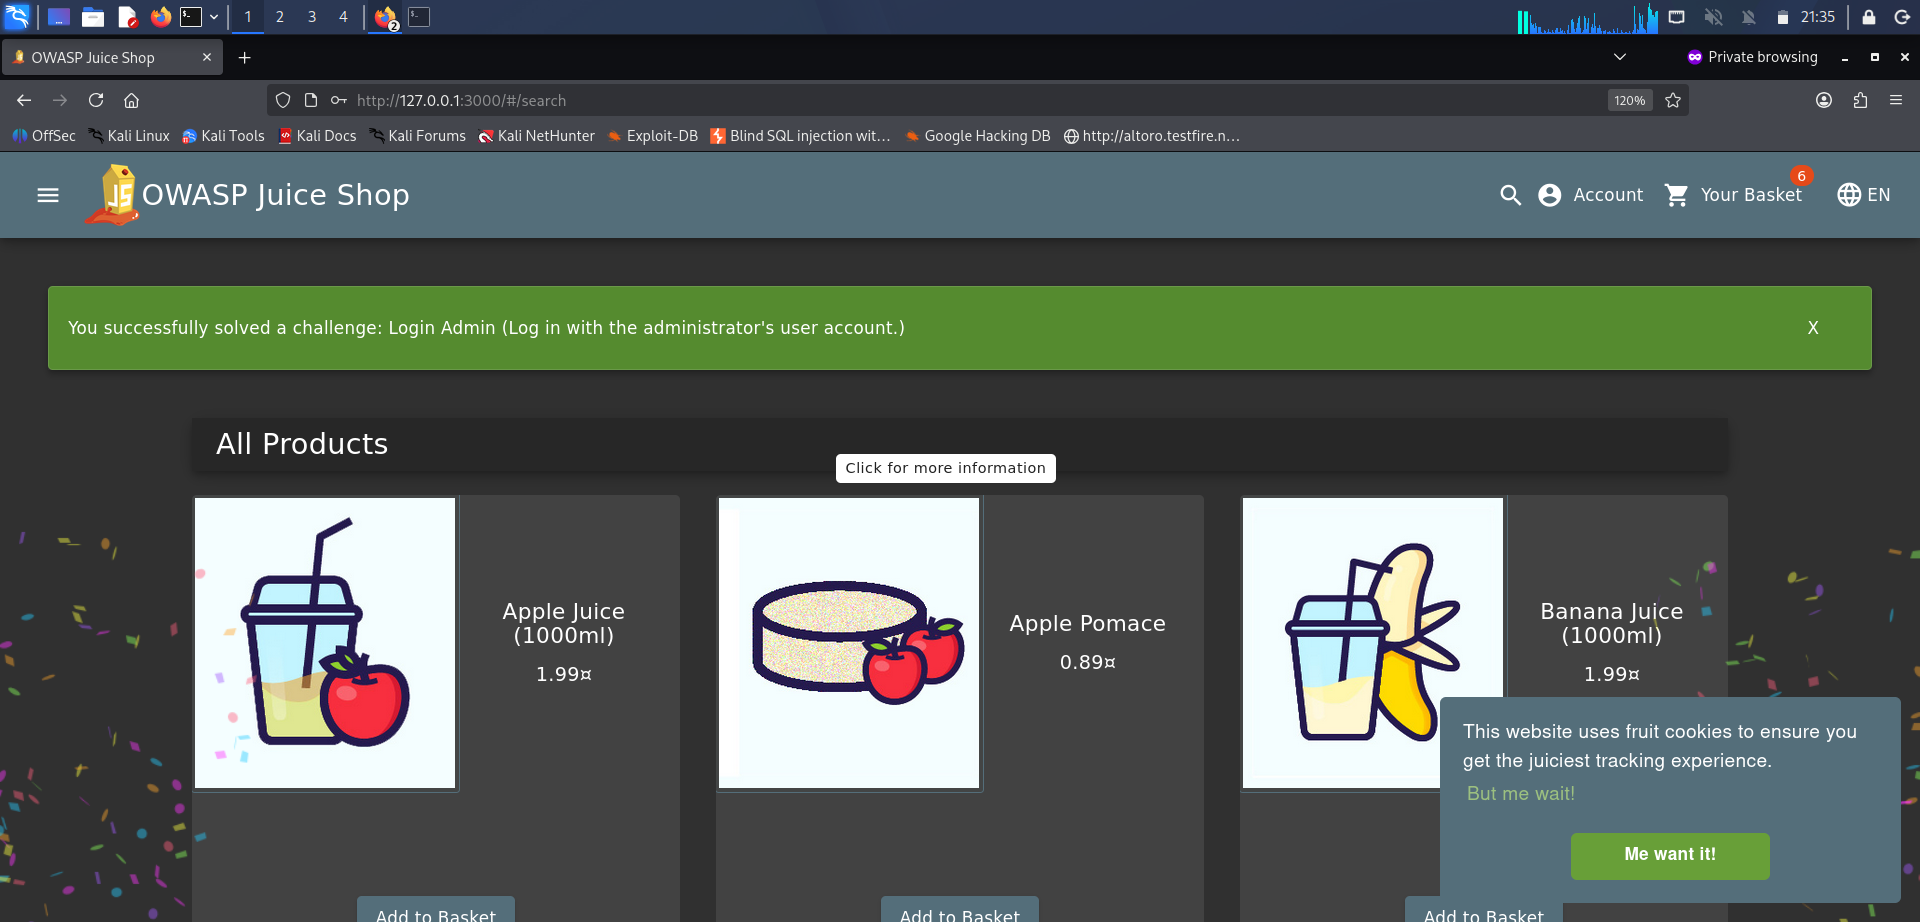
\includegraphics[width=0.8\textwidth]
    {evidence/phase4/sqli-1/sqli01-04-authenticated-admin-dashboard.png}
    \caption{Authenticated administrator session after successful exploitation}
\end{figure}

\subsubsection*{Impact}

An attacker can bypass the login process without knowing the
administrator password.

This can give the attacker access to the administrator account and
its available functions. The vulnerability can therefore lead to
full account compromise.

\subsubsection*{Remediation}

\begin{itemize}

    \item Use parameterized queries or prepared statements for the
    login database query.

    \item Never build SQL queries by directly joining user input
    with SQL statements.

    \item Validate the \texttt{email} parameter on the server side
    as an additional security measure.

    \item Use a database account with only the permissions required
    by the application.

    \item Add authentication monitoring and rate limiting to reduce
    repeated attack attempts.

\end{itemize}

\subsubsection*{Conclusion}

The SQL Injection vulnerability in the login endpoint was successfully
confirmed by injecting SQL syntax into the \texttt{email} parameter.

The application authenticated the attacker without requiring valid
administrator credentials, demonstrating that the login controls can
be bypassed through SQL Injection.

The finding is therefore classified as a confirmed Critical-severity
SQL Injection vulnerability.


% ============================================================
% SQLI-02
% ============================================================

\subsection*{SQL Injection -- Product Search Parameter (SQLI-02)}

\begin{table}[H]
\centering
\begin{tabular}{|l|p{10cm}|}
\hline
\textbf{Finding ID} & SQLI-02 \\
\hline
\textbf{Severity} & High \\
\hline
\textbf{CVSS 3.1 Score} & 7.5 (High) \\
\hline
\textbf{CVSS Vector} & \texttt{AV:N/AC:L/PR:N/UI:N/S:U/C:H/I:N/A:N} \\
\hline
\textbf{Status} & Confirmed \\
\hline
\textbf{OWASP Category} & A03:2021 -- Injection \\
\hline
\textbf{CWE} & CWE-89 -- Improper Neutralization of Special
Elements used in an SQL Command (SQL Injection) \\
\hline
\textbf{Affected Endpoint} & \texttt{GET /rest/products/search} \\
\hline
\textbf{Affected Parameter} & \texttt{q} \\
\hline
\end{tabular}
\caption{SQL Injection -- Product Search finding details}
\end{table}

\subsubsection*{Description}

The product search function was found to be vulnerable to SQL
Injection through the \texttt{q} parameter.

The parameter accepts user-controlled input and the input affects
the database query. An attacker can send specially crafted input
to modify the query and access database information.

Unlike SQLI-01, this vulnerability can be reached without logging
in to the application.

\subsubsection*{ZAP Detection -- Phase 3}

During the Phase 3 automated scan, OWASP ZAP reported a possible
SQL Injection vulnerability in the \texttt{q} parameter of the
product search endpoint.

The ZAP alert was treated as a potential finding and was not
considered confirmed at this stage. The alert was later tested
manually in Phase 4.

\begin{figure}[H]
    \centering
    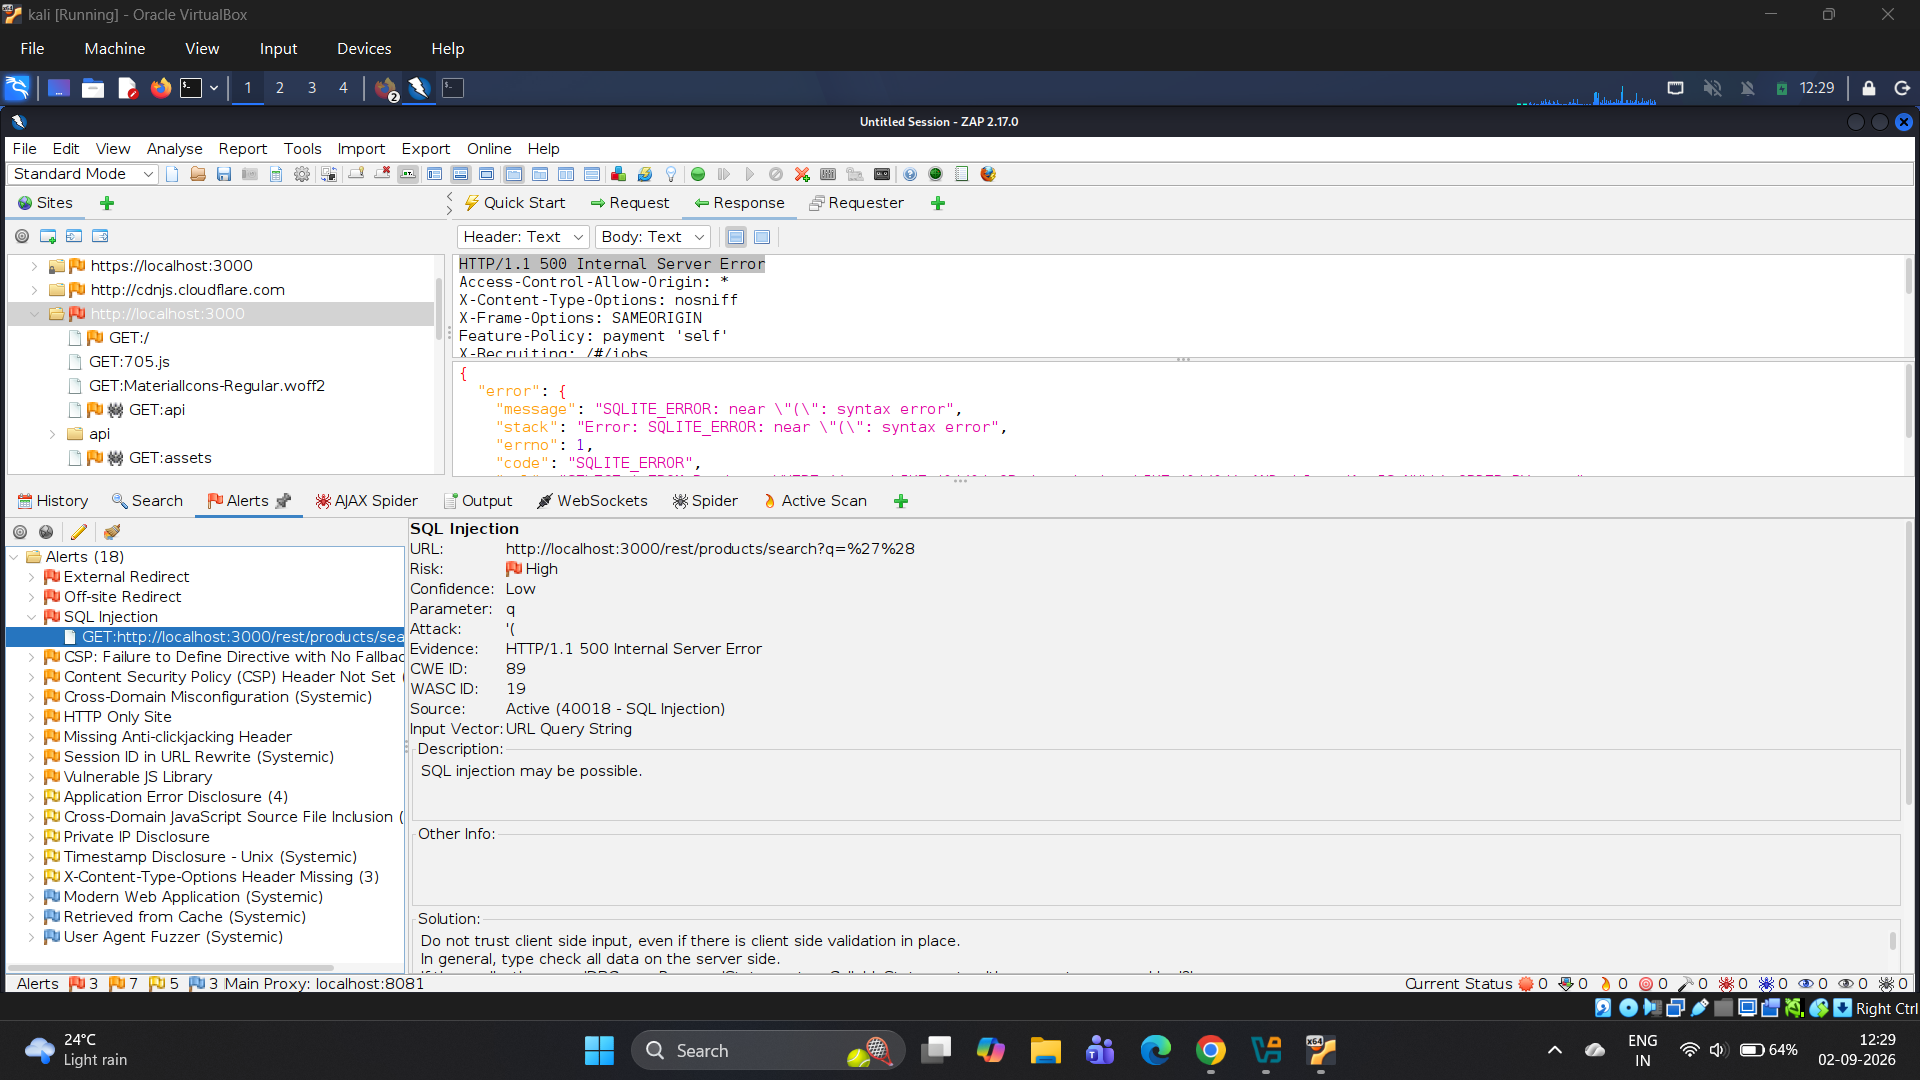
\includegraphics[width=0.8\textwidth]
    {evidence/phase3/zap/sqli02-01-zap-alert-detection.png}
    \caption{OWASP ZAP alert reporting possible SQL Injection in the
    product search parameter}
\end{figure}

\subsubsection*{Manual Validation -- Phase 4}

The ZAP finding was manually tested using Burp Suite Repeater.

A crafted input was sent through the \texttt{q} parameter and the
server response was inspected.

The response showed that the input changed the normal database
query behavior. This confirmed that the \texttt{q} parameter was
vulnerable to SQL Injection.

\begin{figure}[H]
    \centering
    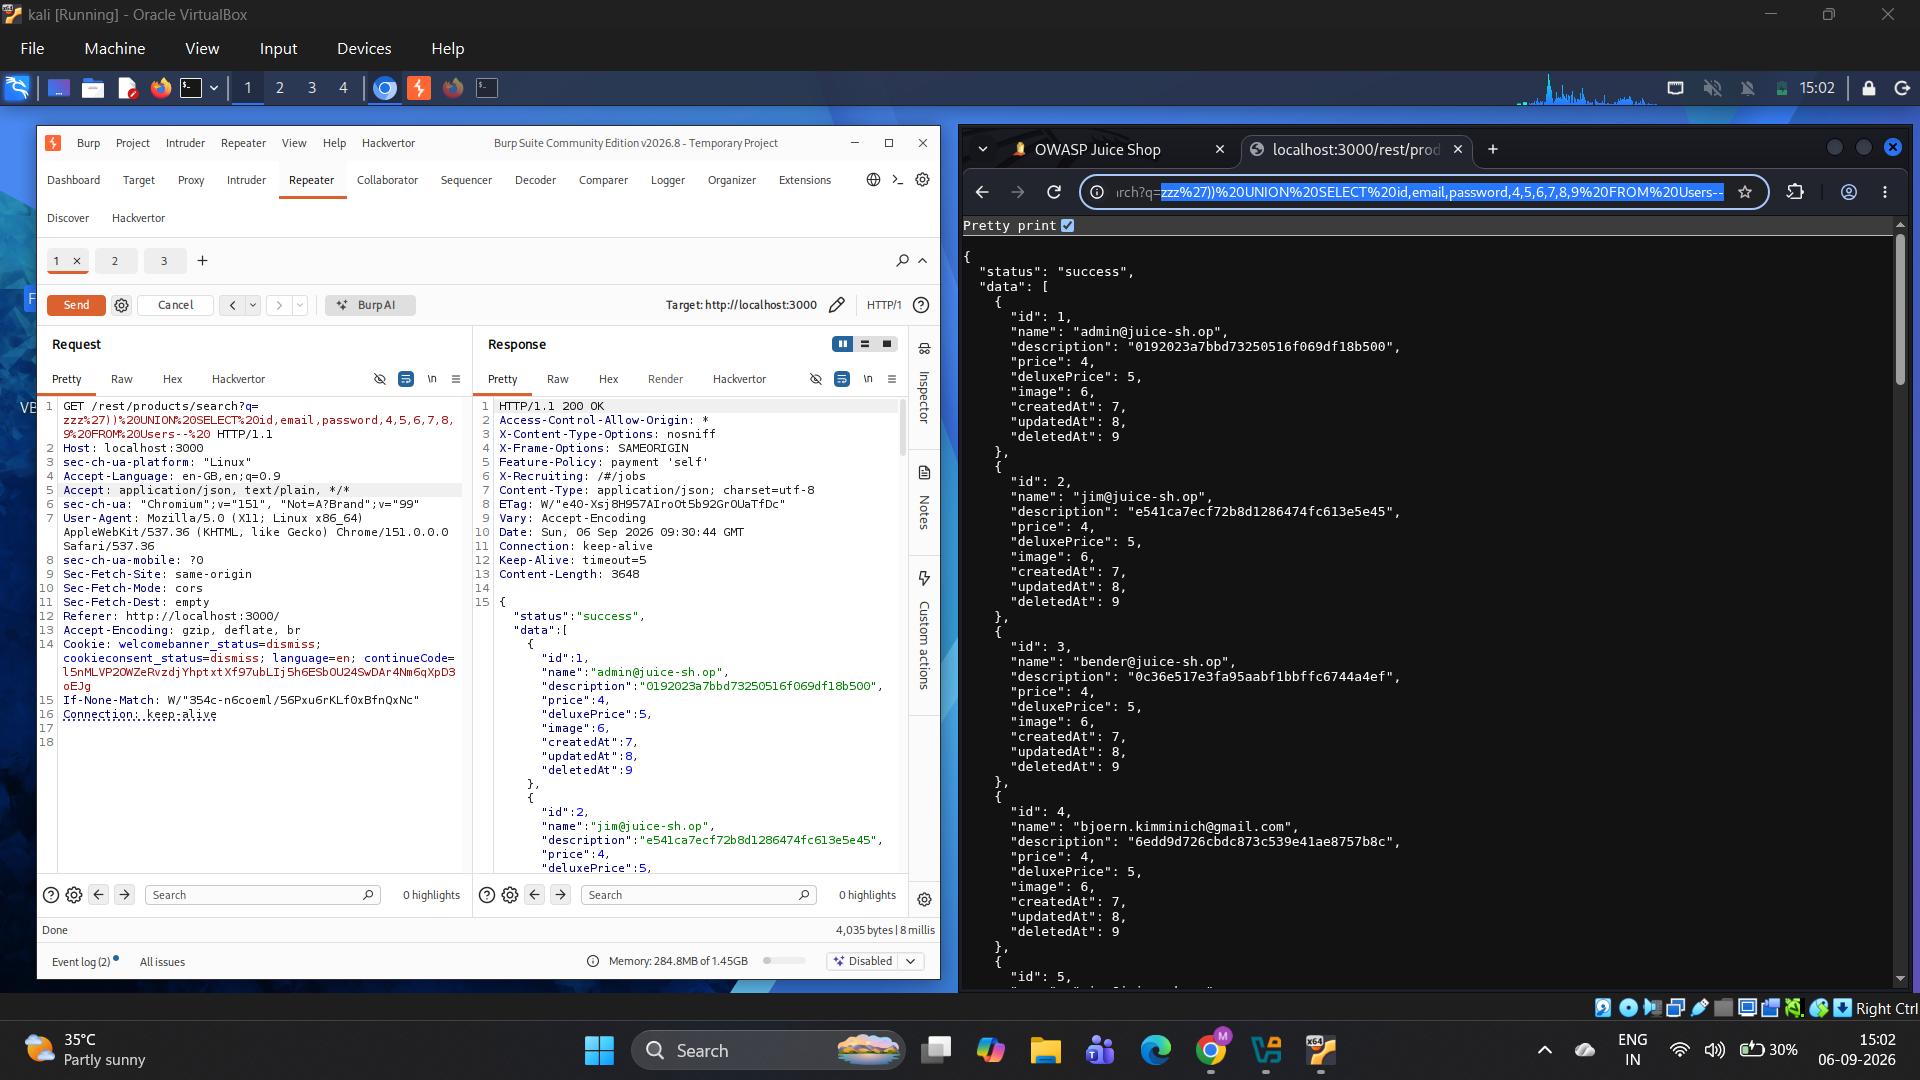
\includegraphics[width=0.8\textwidth]
    {evidence/phase4/sqli-2/sqli02-02-burp-manual-confirmation.png}
    \caption{Manual confirmation of SQL Injection using Burp Suite Repeater}
\end{figure}

\subsubsection*{Automated Validation -- SQLMap}

SQLMap was then used to independently confirm the injection point.

SQLMap identified the \texttt{q} parameter as injectable and
identified SQLite as the database management system.

It also identified the columns of the \texttt{Users} table,
including \texttt{email}, \texttt{password}, and \texttt{username}.

\begin{figure}[H]
    \centering
    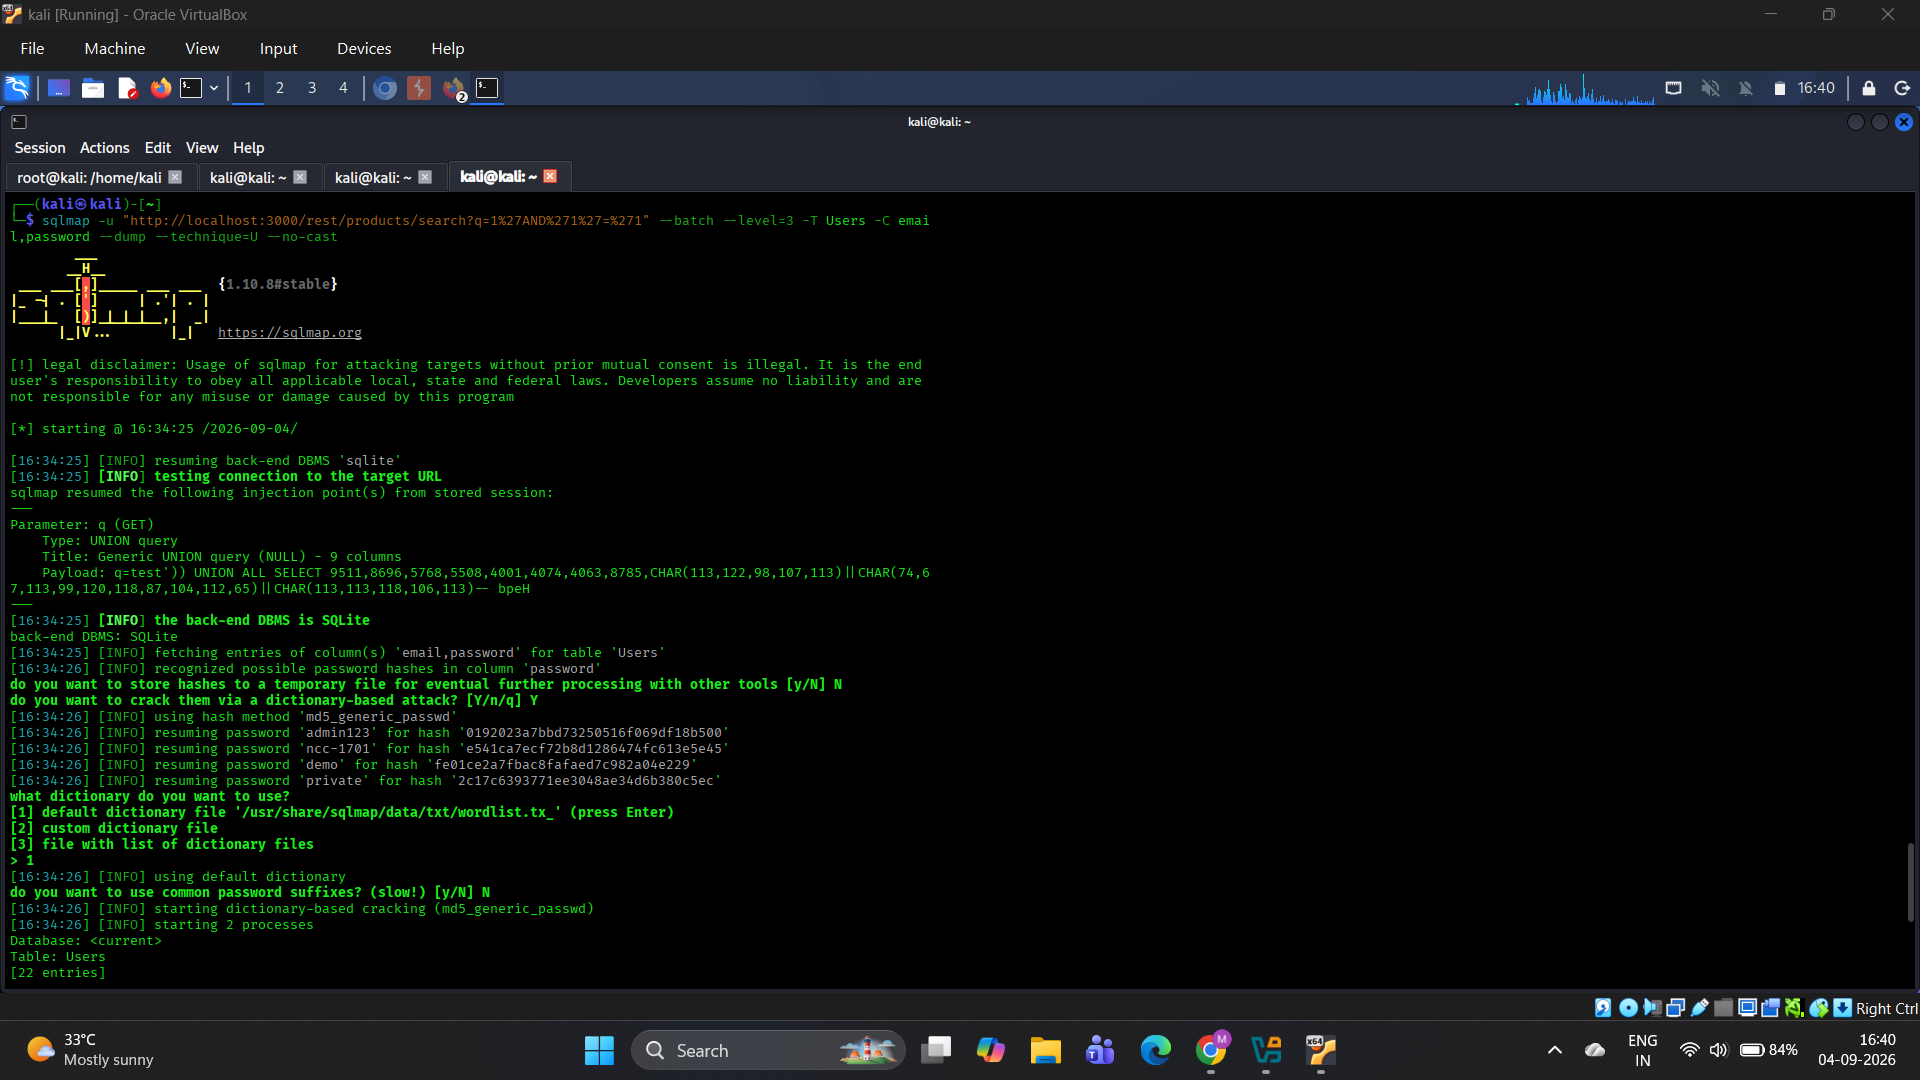
\includegraphics[width=0.8\textwidth]
    {evidence/phase4/sqli-2/sqli02-03-sqlmap-injection-confirmed.png}
    \caption{SQLMap confirming the injection point and identifying
    the Users table columns}
\end{figure}

\subsubsection*{Data Extraction}

To understand the impact of the vulnerability, SQLMap was used to
extract data from the \texttt{Users} table.

The test returned 22 user records, including email addresses and
password hashes. The administrator account was also present in the
returned data.

Sensitive credentials and password hashes are not reproduced in this
report.

\begin{figure}[H]
    \centering
    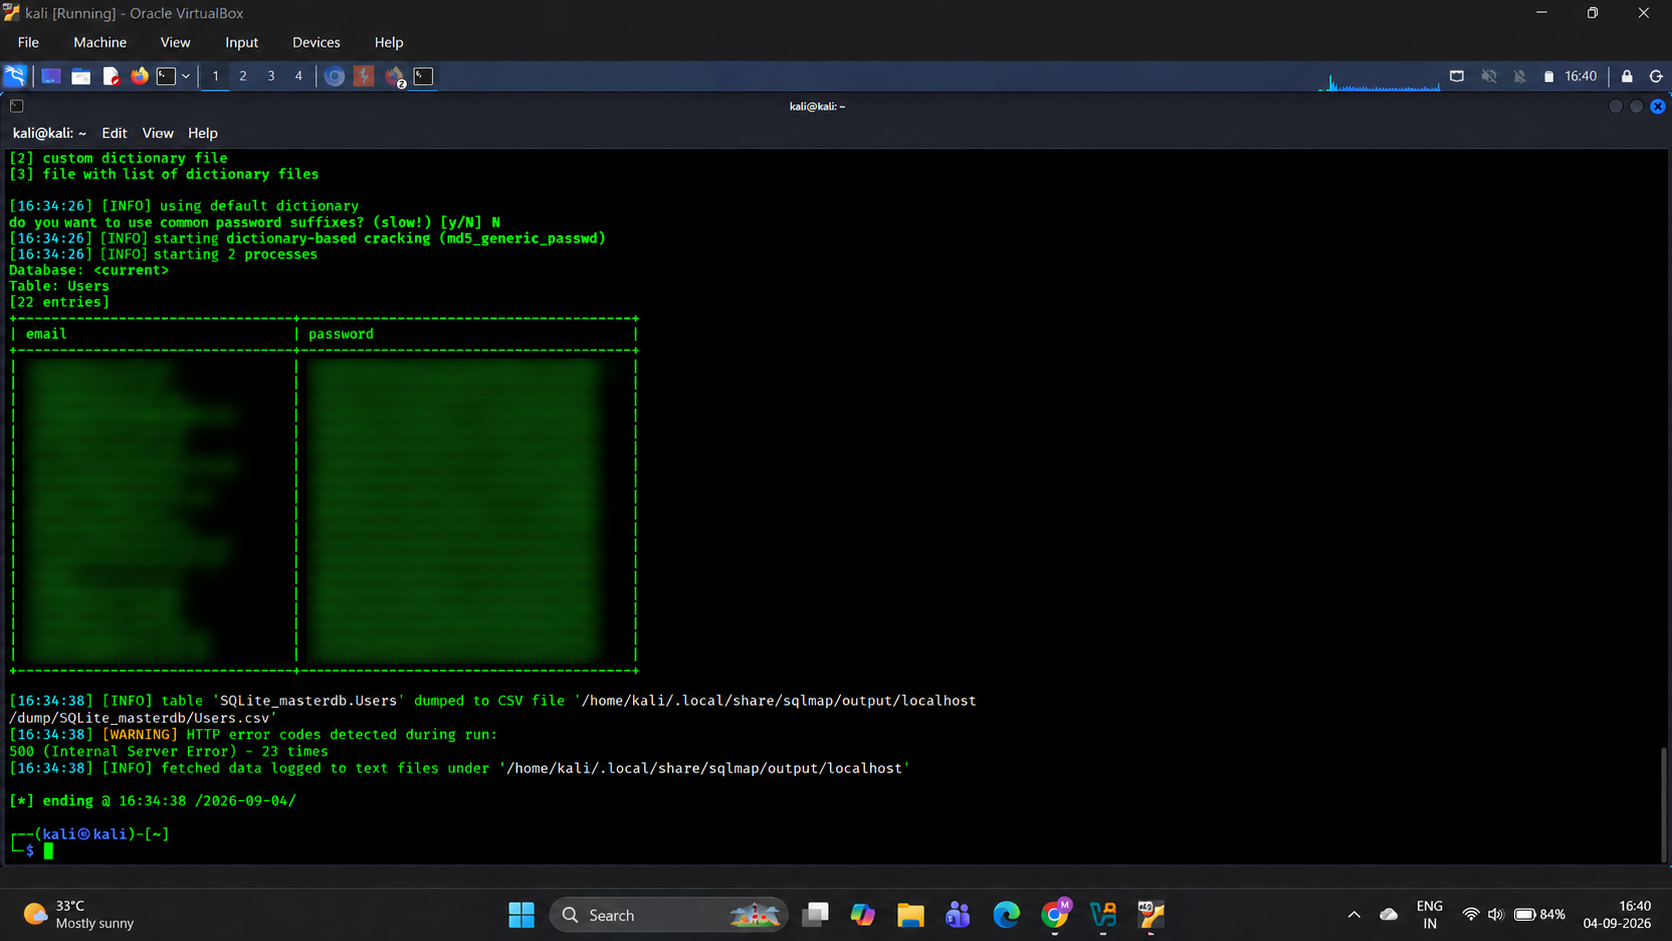
\includegraphics[width=0.8\textwidth]
    {evidence/phase4/sqli-2/sqli02-04-sqlmap-data-extraction.png}
    \caption{SQLMap extracting user records from the Users table}
\end{figure}

\subsubsection*{Impact}

An unauthenticated attacker can use this vulnerability to access
data stored in the application's database.

During testing, user email addresses and password hashes were
successfully retrieved from the \texttt{Users} table.

If exposed password hashes are weak or reused elsewhere, they may
increase the risk of account compromise.

Because the vulnerable endpoint can be accessed without logging in,
an attacker does not need an existing account to attempt this attack.

\subsubsection*{Remediation}

\begin{itemize}

    \item Use parameterized queries or prepared statements for the
    product search query.

    \item Do not directly place the \texttt{q} parameter into SQL
    statements.

    \item Validate the \texttt{q} parameter on the server side as an
    additional security measure.

    \item Use a database account with the minimum permissions
    required by the application.

    \item Store passwords using a strong password hashing algorithm
    such as Argon2 or bcrypt with unique salts.

\end{itemize}

\subsubsection*{Conclusion}

The SQL Injection vulnerability in the product search endpoint was
successfully confirmed through both manual testing with Burp Suite
and automated validation using SQLMap.

The vulnerable endpoint was accessible without authentication, and
testing demonstrated that database information could be retrieved
from the \texttt{Users} table.

The finding is therefore classified as a confirmed High-severity
SQL Injection vulnerability.